%!TEX root = ./main.tex
\documentclass[12pt,letterpaper]{scrartcl}
\usepackage[secthm,mdthm,simplethm]{beel}
%!TEX root = ./main.tex
\usepackage{graphicx}
\usepackage{tcolorbox}
\usepackage[margin=1in,top=0.8in, bottom = 0.8in]{geometry}
%%%%%%Packages%%%%%%%%%%%%%
\usepackage{amsmath}
\usepackage{amsfonts}
\usepackage{amsthm}
\usepackage{amssymb}
\usepackage{array}
\usepackage{comment}
\usepackage{enumitem}
\usepackage{graphicx}
\usepackage{hyperref}
\usepackage[utf8]{inputenc}
\usepackage{mathtools}
\usepackage{multicol}
\usepackage{tabto}
\usepackage{tikz}
\usepackage{pgfplots}
\usepackage{setspace}
\usepackage[all]{xy}
\usepackage{thmtools}
\usepackage{MnSymbol,wasysym}
\usepackage{venndiagram}
\usepackage{listings}
\usetikzlibrary{decorations.pathmorphing,shapes}
%%%%Theorem Enviorment Setup%%%%%%%
\begin{comment}
\theoremstyle{definition}
\newtheorem{theorem}{Theorem}[section]
\newtheorem{corollary}{Corollary}[theorem]
\newtheorem{lemma}[theorem]{Lemma}
\newtheorem{claim}[theorem]{Claim}
\newtheorem{definition}{Definition}[section]
\newtheorem{example}{Example}[section]
\newtheorem{remark}{Remark}[section]
\newtheorem{proposition}[theorem]{Proposition}
\end{comment}
\pgfplotsset{compat = 1.15}
%%%%%%%%%HyperLink Setup%%%%%%%%%%%
%
%%%%%%%%%%%%%%%Commands%%%%%%%%%%%%%%%%
\newcommand{\pml}{\begin{pmatrix}}
\newcommand{\pmr}{\end{pmatrix}}
\newcommand{\bml}{\left[ \begin{array}{ccccccccccccccccccccccccccccccccccccccccccccccccccccccccccc}}
\newcommand{\bmr}{\end{array} \right]}
\newcommand{\aml}{\left[ \begin{array}{rrr|r}}
\newcommand{\amr}{\end{array} \right]}
\newcommand{\vml}{\left\vert \begin{array}{rrrrrrrrrr}}
\newcommand{\vmr}{\end{array} \right\vert}
\renewcommand{\tab}{\hspace{1cm}}
\renewcommand{\b}{\mathbb}
\renewcommand{\c}{\mathcal}
\newcommand{\lb}{\left\{}
\newcommand{\rb}{\right\}}
\newcommand{\la}{\langle}
\newcommand{\ra}{\rangle}
\renewcommand{\bar}{\overline}
\newcommand{\ngroup}{\trianglelefteq}
\newcommand{\ver}{ \ | \ }
\renewcommand{\t}{\text}
\newcommand{\z}{\mathbb Z}
\renewcommand{\r}{\mathbb R}
\newcommand{\q}{\mathbb Q}
\newcommand{\ex}{\textbf{Example. }}
\renewcommand{\mod}[1]{\t{ (mod } {#1})}
\newcommand{\zz}[1]{\b Z/ {#1} \b Z}
\newcommand{\cg}[1]{\la {#1} \ra}
\newcommand{\li}[2]{{#1}_1,{#1}_2, \ldots, {#1}_{#2} }
\renewcommand{\v}{\vec}
\renewcommand{\t}{\tilde}
\newcommand{\spa}{\text{span}}
\newcommand{\lincomb}[3]{{#1}_1{#2}_1 + {#1}_2{#2}_2 + \cdots + {#1}_{#3}{#2}_{#3}}
\newcommand{\nul}{\text{Null }}
\newcommand{\col}{\text{Col }}
\newcommand{\range}{\text{Range }}
\newcommand{\itab}{\hspace{-0.25cm}}
\newcommand{\omicron}{o}
\renewcommand{\qedsymbol}{$\blacksquare$}
\renewcommand{\vec}{\mathbf}
\renewcommand{\Re}{\textrm{Re}}
\renewcommand{\Im}{\textrm{Im}}
%%%%%%%%%%%% main doc%%%%%%%%%%%%
\begin{document}
\thispagestyle{empty}
$ $
\vfill$\circ$
\begin{center}
\centerline{\huge \textbf{CS 170, Fall 2022}} 
\end{center}
\vfill
$ $
\newpage
\tableofcontents
\newpage
\renewcommand\thesubsection{\thesection.\alph{subsection}}
\renewcommand\thesubsubsection{\thesection.\roman{subsubsection}}
\section{Algorithms with numbers} \vfill
\section{Divide-and-conquer Algorithms}

\subsection{Multiplication}

\begin{definition}[Integer Multiplication]
A divide-and-conquer algorithm for integer multiplication is defined as follows:
\begin{lstlisting}[mathescape=true, language=Octave]
function mul(x(0b[1...k]), y(0b[1...h]))
	%Input: Positive integers x, y in binary
	%Output: x times y

	n = $\max$(size of x, size of y)
	if n == 1: return $x\times y$

	$x_L$, $x_R$ = x(0b[1...$\lceil n/2\rceil$]), x(0b[$\lfloor n/2\rfloor$...n])
	$y_L$, $y_R$ = y(0b[1...$\lceil n/2\rceil$]), y(0b[$\lfloor n/2\rfloor$...n])

	$P_1 = mul(x_L, y_L)$
	$P_2 = mul(x_R, y_R)$
	$P_3 = mul(x_L+x_R, y_L+y_R)$
	return $P_1\times 2^n + (P_3-P_1-P_2)\times 2^{n/2}+P_2$
\end{lstlisting}
Where $0b[1...k]$ denotes the binary string representing a number.
\end{definition}
Each call of \textit{mul} has three recursive calls, inputs of which are half the size of the original inputs, and the base cases (x times y) take constant time. Therefore we conclude that the time taken by this algorithm is
\[
T(n) = 3T(n/2)+O(n)
\]
Apply the Master Algorithm in Chap 2.b, we conclude that the time complexity of this algorithm is
\[
T(n) \in \Theta(n^{\log_23}) \approx \Theta(n^{1.585})
\]

\subsection{Recurrence Relations}

\begin{theorem}[Master Algorithm]
If $T(n) = aT(n/b) + cn^k$ and $T(1) = c$ for some constants $a$, $b$, $c$ and $k$, then
\begin{equation*}
T(n) \in \begin{cases}
\Theta(n^k) &if \; a<b^k \\
\Theta(n^k\log n) &if \; a=b^k \\
\Theta(n^{\log_ba}) &if \; a>b^k
\end{cases}
\end{equation*}
\end{theorem}

\subsection{Mergesort}

\begin{definition}[Mergesort]
The Mergesort algorithm is defined as follows:
\begin{lstlisting}[mathescape=true, language=Octave]
function mergesort(a[1...n])
	%Input: An array of numbers a[1...n]
	%Output: Sorted array a

	if n>1:
		return merge(mergesort(a[1...$\lfloor n/2 \rfloor$]), mergesort(a[$\lfloor n/2 \rfloor$+1...n]))
	else:
		return a

function merge(x[1...k], y[1...h])
	%Input: Two arrays of numbers (x[1...k], y[1...h])
	%Output: An array of numbers in x and y in ascending order

	if k=0: return y
	if l=0: return x
	if x[1] <= y[1]:
		return x[1] $\circ$ merge(x[2...k], y[1...h])
	else:
		return y[1] $\circ$ merge(x[1...k], y[2...h])
\end{lstlisting}
Where $\circ$ denotes concatenation.
\end{definition}

The \textit{merge} function above does a constant amount of work (concatenating two arrays) per recursive call, for a total running time of $O(k + h)$. Thus the calls to \textit{merge} in \textit{mergesort} are linear, we conclude that the overall time taken by \textit{mergesort} is
\[
T(n) = 2T(n/2) + O(n)
\]
Recall the Master Algorithm in Chap 2.b, we conclude that the time complexity of this algorithm is
\[
T(n) \in \Theta(n\log n)
\]

\begin{remark}
$n\log n$ is the lower bound for sorting, and therefore \textit{mergesort} is optimal.

\begin{proof}
Sorting algorithms can be depicted as trees that each non-leaf node represents a comparison between two elements, and each leaf denotes a permutation of the input array (and thus a binary search tree since each non-leaf nodes have two children). Consider such tree that sorts an array $a[1...n]$. The total number of the leaves is $n!$. A binary tree of depth $d$ has at most $2^d$ leaves. Therefore, the depth of the tree and the complexity of this algorithm should be at least $\log(n!)$, which is the worst case of this algorithm. Since $\log(n!)\le cn\log(n)$, we conclude that $n\log(n)$ is optimal for sorting algorithms.
\end{proof}
\end{remark}

\subsection{Medians}

\begin{definition}[selection]
A randomized divide-and-conquer algorithm for selection is defined as follows

\end{definition}

\subsection{Matrix Multiplication}

\begin{definition}

\end{definition}

\subsection{Fast Fourier Transform} \vfill
% \section{Decomposition of Graphs}

\subsection{DFS in Undirected Graphs}

\begin{definition}[explore]
Finding all nodes reachable from a particular node.
	\begin{lstlisting}[mathescape=true, language=Octave]
procedure explore(G, v):
	% Input: Graph G = (V, E), v a node in V
	% Output: u.visited is set true for all node u reachable from v
	v.visited = true
	previsit(v)
	foreach (v, u) in E:
		if not u.visited: explore(G, u)
	postvisit(v)
\end{lstlisting}
Where previsit(v) and postvisit(v) denotes the "time" $\tau$ before and after v is explored, respectively.
\end{definition}

\begin{definition}[DFS]
Based on Definition of explore, a DFS procedure is as follows:
\begin{lstlisting}[mathescape=true, language=Octave]
procedure DFS(G)
	% Input: Graph G = (V, E)
	forall v in V:
		if not v.visited: explore(v)
\end{lstlisting}
\end{definition}

\begin{definition}[ordering]
The previsit and postvisit ordering is defined as follows:
\begin{lstlisting}[mathescape=true, language=Octave]
procedure previsit(v)
	pre[v] = clock
	clock += 1
procedure postvisit(v)
	post[v] = clock
	clock += 1
\end{lstlisting}
\end{definition}[visit orderings]

\begin{remark}
The implementation of a DFS uses a stack and DFS's runtime is $O(|V|+|E|)$.
\end{remark}

\subsection{DFS in Directed Graphs}

\begin{definition}[Type of Edges]
There four types of edges:
\begin{itemize}
	\item Tree edges are part of the DFS forest
	\item Forward edges lead to a nonchild descendant
	\item Back edges lead to a not-direct ancestor
	\item Cross edges lead to a node that is neither descendant nor ancestor, a node that has already been completely explored.
\end{itemize}
An edge (u, v) in E is:
\begin{itemize}
	\item Forward if pre(u) $<$ pre(v) $<$ post(v) $<$ post(u)
	\item Back if pre(v) $<$ pre(u) $<$ post(u) $<$ post(v)
	\item Cross if pre(v) $<$ post(v) $<$ pre(u) $<$ post(u)
\end{itemize}
\end{definition}

\begin{definition}
	A directed graph has a cycle iff its DFS reveals a back edge. If the DFS of a directed graph reveals no back edge, the graph is a Directed Acyclic Graph (DAG).
\end{definition}

\begin{remark}
	In a DF traverse of a binary tree, the visiting order of nodes can be found by labeling the graph like follows: \\
	\begin{center}
		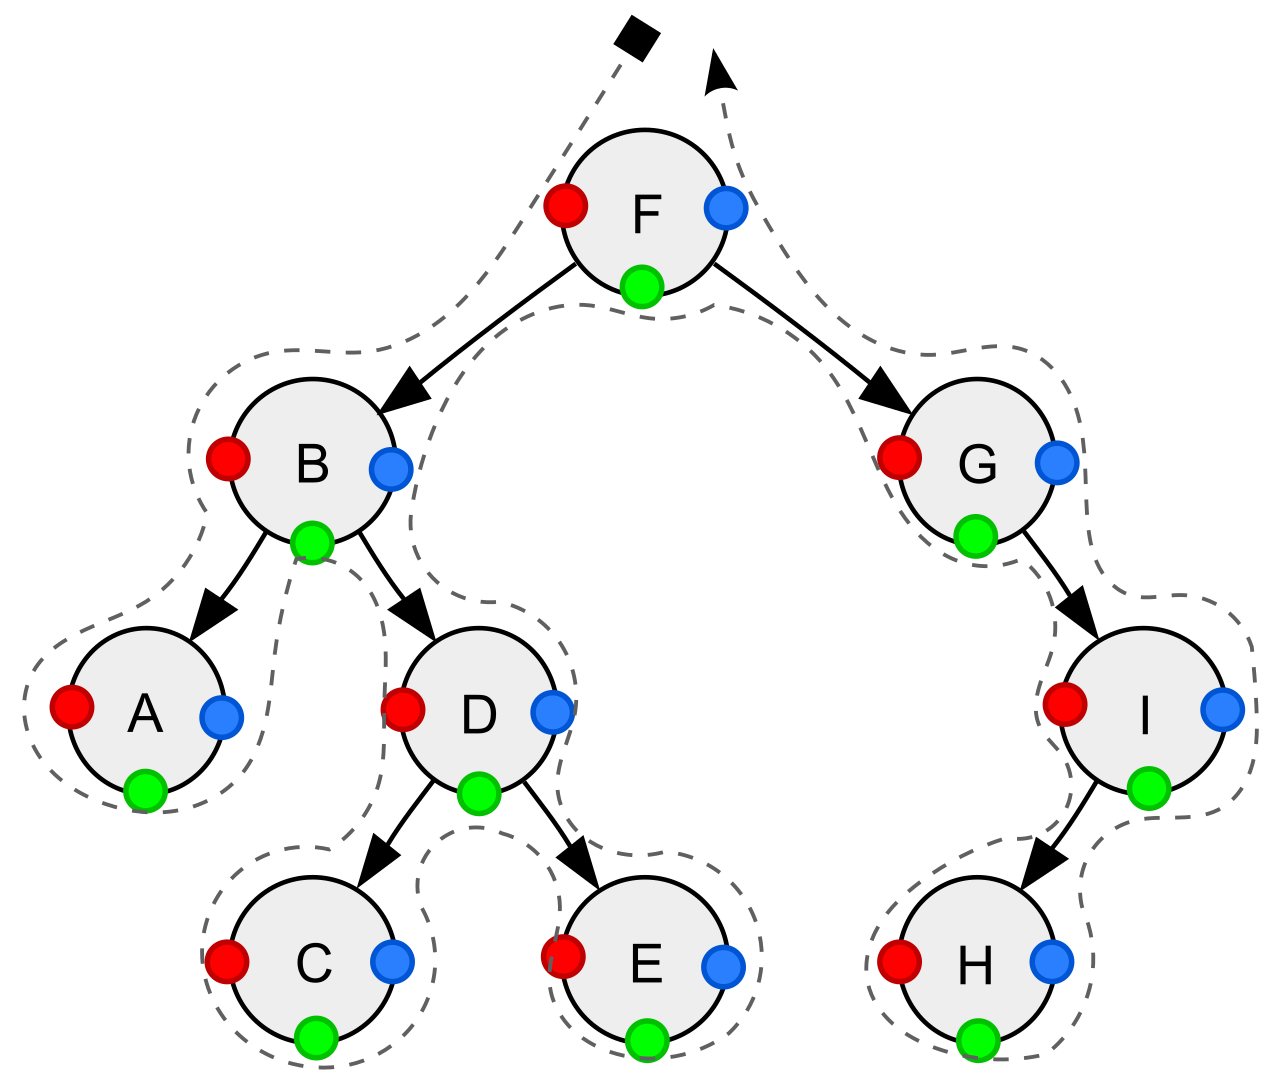
\includegraphics[scale=0.2]{images/dfs_order.png} \\
	\end{center}
	Where red dots denote preorder, green dots denote in-order, and blue dots denote post-order.
\end{remark}

\begin{remark}
	Topological sort: if G(V, E) is a DAG with (u, v) in E, then post(u) > post(v)
\end{remark}

\subsection{Strongly Connected Components} \vfill
% \section{Paths in Graphs}

\subsection{Distances}

\subsection{BFS}

\subsection{Lengths on Edges}

\subsection{Dijkstra's}

\subsection{Priority Queue Implementation}

\subsection{Shortest Paths in the Presence of Negative Edges}

\subsection{Shortest Paths in DAGs}
 \vfill
% \include{chap5} \vfill
% \include{chap6} \vfill
% \include{chap7} \vfill
% \include{chap8} 

\end{document}